\documentclass[tikz,border=20pt]{standalone}
\usetikzlibrary{calc,arrows.meta,shapes}
\usepackage{xcolor}

\definecolor{wallcolor}{HTML}{F0E6D8}
\definecolor{skirtcolor}{HTML}{6B4423}
\definecolor{floorcolor}{HTML}{9C6644}
\definecolor{rugcolor}{HTML}{DDB892}
\definecolor{curtainrose}{HTML}{B56576}
\definecolor{chairteal}{HTML}{5C6B73}
\definecolor{grandmacard}{HTML}{D88C9A}
\definecolor{grandmashawl}{HTML}{F6BD60}
\definecolor{blanketgreen}{HTML}{84A59D}
\definecolor{woodtable}{HTML}{8B5E34}
\definecolor{teacup}{HTML}{E9EDC9}
\definecolor{nightsky}{HTML}{1D2D44}

\begin{document}
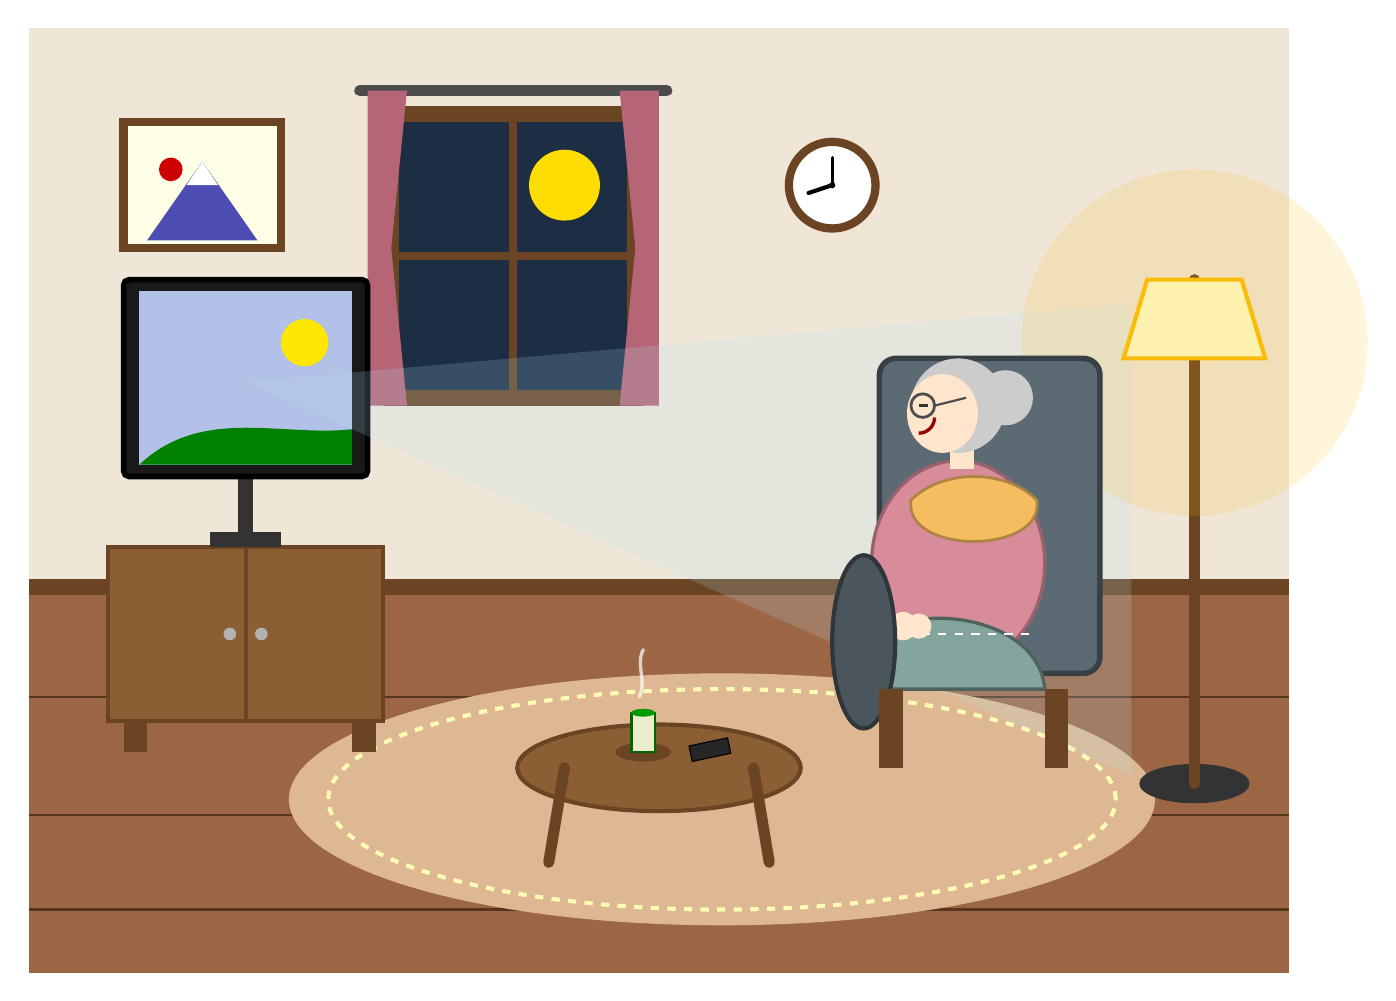
\begin{tikzpicture}[x=1cm, y=1cm]

  % Background Wall & Floor
  \fill[wallcolor] (-8, -1) rectangle (8, 6);
  \fill[skirtcolor] (-8, -1.2) rectangle (8, -1);
  \fill[floorcolor] (-8, -6) rectangle (8, -1.2);

  % Floor perspective lines
  \draw[skirtcolor!80!black, line width=1pt] (-8, -2.5) -- (8, -2.5);
  \draw[skirtcolor!80!black, line width=1pt] (-8, -4.0) -- (8, -4.0);
  \draw[skirtcolor!80!black, line width=1pt] (-8, -5.2) -- (8, -5.2);

  % Window with Moon (Left background)
  \fill[skirtcolor] (-3.5, 1.2) rectangle (-0.2, 5.0);
  \fill[nightsky] (-3.3, 1.4) rectangle (-0.4, 4.8);
  \fill[yellow!80!orange] (-1.2, 4.0) circle (0.45);
  \draw[skirtcolor, line width=3pt] (-1.85, 1.4) -- (-1.85, 4.8);
  \draw[skirtcolor, line width=3pt] (-3.3, 3.1) -- (-0.4, 3.1);

  % Curtain Rod & Curtains
  \draw[black!70, line width=4pt, line cap=round] (-3.8, 5.2) -- (0.1, 5.2);
  \fill[curtainrose] (-3.7, 5.2) -- (-3.2, 5.2) -- (-3.4, 3.2) -- (-3.2, 1.2) -- (-3.7, 1.2) -- cycle;
  \fill[curtainrose] (0.0, 5.2) -- (-0.5, 5.2) -- (-0.3, 3.2) -- (-0.5, 1.2) -- (0.0, 1.2) -- cycle;

  % Wall Art Frame
  \draw[skirtcolor, fill=yellow!10, line width=3pt] (-6.8, 3.2) rectangle (-4.8, 4.8);
  \fill[blue!40!gray] (-6.5, 3.3) -- (-5.8, 4.3) -- (-5.1, 3.3) -- cycle;
  \fill[white] (-6.0, 4.0) -- (-5.8, 4.3) -- (-5.6, 4.0) -- cycle;
  \fill[red!80!black] (-6.2, 4.2) circle (0.15);

  % Wall Clock
  \draw[skirtcolor, fill=white, line width=3pt] (2.2, 4.0) circle (0.55);
  \fill[black] (2.2, 4.0) circle (0.04);
  \draw[black, line width=1.5pt, line cap=round] (2.2, 4.0) -- (1.9, 3.9);
  \draw[black, line width=1.2pt, line cap=round] (2.2, 4.0) -- (2.2, 4.35);

  % Floor Oval Rug
  \fill[rugcolor] (0.8, -3.8) ellipse (5.5 and 1.6);
  \draw[yellow!30!white, dashed, line width=1.5pt] (0.8, -3.8) ellipse (5.0 and 1.4);

  % TV Setup (Left Foreground)
  % TV Cabinet
  \filldraw[fill=woodtable, draw=skirtcolor, line width=1.5pt] (-7.0, -2.8) rectangle (-3.5, -0.6);
  \draw[skirtcolor, line width=1.5pt] (-5.25, -2.8) -- (-5.25, -0.6);
  \fill[black!30] (-5.45, -1.7) circle (0.08);
  \fill[black!30] (-5.05, -1.7) circle (0.08);
  \fill[skirtcolor] (-6.8, -3.2) rectangle (-6.5, -2.8);
  \fill[skirtcolor] (-3.9, -3.2) rectangle (-3.6, -2.8);

  % TV Stand & Screen
  \fill[black!80] (-5.7, -0.6) rectangle (-4.8, -0.4);
  \fill[black!80] (-5.35, -0.4) rectangle (-5.15, 0.3);
  \filldraw[fill=black!90, draw=black, line width=2pt, rounded corners=2pt] (-6.8, 0.3) rectangle (-3.7, 2.8);
  \fill[cyan!40!blue!30] (-6.6, 0.45) rectangle (-3.9, 2.65);
  % Broadcast landscape on screen
  \fill[green!50!black] (-6.6, 0.45) .. controls (-5.8, 1.2) and (-4.8, 0.8) .. (-3.9, 0.9) -- (-3.9, 0.45) -- cycle;
  \fill[yellow!90!orange] (-4.5, 2.0) circle (0.3);

  % Soft TV Glow Triangle towards Grandma
  \fill[cyan!30, opacity=0.18] (-5.25, 1.5) -- (6.0, 2.5) -- (6.0, -3.5) -- cycle;

  % Floor Lamp (Far Right)
  \fill[black!80] (6.8, -3.6) ellipse (0.7 and 0.25);
  \draw[skirtcolor, line width=4pt, line cap=round] (6.8, -3.6) -- (6.8, 2.8);
  \fill[yellow!20, draw=yellow!50!orange, line width=1.5pt]
    (6.2, 2.8) -- (7.4, 2.8) -- (7.7, 1.8) -- (5.9, 1.8) -- cycle;
  \fill[yellow!50!orange, opacity=0.15] (6.8, 2.0) circle (2.2);

  % Armchair & Grandmother (Right)
  % Armchair Back & Wing
  \filldraw[fill=chairteal, draw=chairteal!60!black, line width=2pt, rounded corners=6pt]
    (2.8, -2.2) rectangle (5.6, 1.8);

  % Grandmother Torso & Cardigan
  \filldraw[fill=grandmacard, draw=grandmacard!70!black, line width=1.2pt]
    (3.8, -0.8) ellipse (1.1 and 1.3);

  % Shawl over shoulders
  \filldraw[fill=grandmashawl, draw=grandmashawl!70!black, line width=1pt]
    (3.2, 0.0) .. controls (3.6, 0.4) and (4.4, 0.4) .. (4.8, 0.0)
    .. controls (4.9, -0.7) and (3.1, -0.7) .. (3.2, 0.0) -- cycle;

  % Green blanket over knees
  \filldraw[fill=blanketgreen, draw=blanketgreen!60!black, line width=1.2pt]
    (2.5, -2.4) .. controls (2.2, -1.2) and (4.8, -1.2) .. (4.9, -2.4) -- cycle;
  \draw[white!70, dashed, line width=1pt] (2.7, -1.7) -- (4.7, -1.7);

  % Hands folded gently on lap
  \fill[orange!20!white] (3.1, -1.6) circle (0.18);
  \fill[orange!20!white] (3.3, -1.6) circle (0.16);

  % Neck & Head (turned left toward TV)
  \fill[orange!20!white] (3.7, 0.4) rectangle (4.0, 0.9);
  % Hair bun
  \fill[gray!40] (4.4, 1.3) circle (0.35);
  % Head
  \fill[gray!40] (3.8, 1.2) circle (0.6);
  \fill[orange!20!white] (3.6, 1.1) ellipse (0.45 and 0.5);
  % Glasses
  \draw[black!70, line width=1pt] (3.35, 1.2) circle (0.15);
  \draw[black!70, line width=0.8pt] (3.5, 1.2) -- (3.9, 1.3);
  % Eye looking at TV
  \draw[black!80, line width=1.2pt] (3.3, 1.2) -- (3.42, 1.2);
  % Gentle smile
  \draw[red!60!black, line width=1.2pt] (3.3, 0.85) arc (-90:0:0.2);

  % Armchair Front Arm & Legs
  \filldraw[fill=chairteal!80!black, draw=chairteal!50!black, line width=1.5pt]
    (2.6, -1.8) ellipse (0.4 and 1.1);
  \fill[skirtcolor] (2.8, -3.4) rectangle (3.1, -2.4);
  \fill[skirtcolor] (4.9, -3.4) rectangle (5.2, -2.4);

  % Coffee Table & Tea Cup (Center Foreground)
  \filldraw[fill=woodtable, draw=skirtcolor, line width=1.5pt] (0.0, -3.4) ellipse (1.8 and 0.55);
  \draw[skirtcolor, line width=4pt, line cap=round] (-1.2, -3.4) -- (-1.4, -4.6);
  \draw[skirtcolor, line width=4pt, line cap=round] (1.2, -3.4) -- (1.4, -4.6);

  % Tea Cup (Yunomi)
  \fill[skirtcolor] (-0.2, -3.2) ellipse (0.35 and 0.12);
  \filldraw[fill=teacup, draw=green!40!black, line width=0.8pt]
    (-0.35, -3.2) rectangle (-0.05, -2.7);
  \fill[green!60!black] (-0.2, -2.7) ellipse (0.15 and 0.05);
  % Steam wisps
  \draw[white, opacity=0.7, line width=1.2pt, line cap=round]
    (-0.25, -2.5) .. controls (-0.15, -2.3) and (-0.3, -2.1) .. (-0.2, -1.9);

  % Remote on table
  \filldraw[fill=black!85, draw=black, rotate around={12:(0.5,-3.2)}] (0.4, -3.3) rectangle (0.9, -3.1);

\end{tikzpicture}
\end{document}
